\documentclass{sintefbeamer}

% packages, font, color, and newcommands
\usepackage{amsfonts, amsmath, oldgerm, lmodern, bm}
% \usepackage[font={footnotesize}]{caption}
\usepackage{natbib}
\usepackage{url}
\usepackage{tikz}
\usepackage{amssymb}
\usepackage{amsmath}
\usepackage{amsthm}
\usepackage{mathrsfs}
\usepackage{empheq}
\usepackage{mdframed}
\usepackage{bm}
\usepackage{animate}
\usepackage{xcolor,colortbl}
\usepackage{graphicx}
%\usepackage{dot2texi}
% \usepackage{dot2texi}
\usepackage{tikz}
\usetikzlibrary{shapes,arrows}

\bibliographystyle{apalike}
\usefonttheme{serif}
\usetikzlibrary{calc}
\definecolor{carminered}{rgb}{1.0, 0.0, 0.22}
\definecolor{burgundy}{rgb}{0.5, 0.0, 0.13}
\title{Averaged equations for a buoyancy driven suspension of droplets}
\subtitle{Discussion Marc Massot}
\author{N. Fintzi \footnote{IFP \'Energies Nouvelles, France}$^{,2}$,S. Popinet\footnote{Sorbonne Universit\'e, France}, and \underline{JL. Pierson$^1$}}
% \date{Created on May 22, 2022}
\definecolor{burntorange}{rgb}{0.8, 0.33, 0.0}
\titlebackground{image/800good.png}


% document body
\addtobeamertemplate{navigation symbols}{}{%
    \usebeamerfont{footline}%
    \usebeamercolor[fg]{footline}%
    % \hspace{1em}%
    % \vspace{1em}%
    \insertframenumber/\inserttotalframenumber
}
\usepackage{stmaryrd}


\begin{document}
\maketitle
\section*{}

\begin{frame}
  \frametitle{Objectives and motivation}



\textbf{Euler-Euler} modeling of dispersed two phase flows 
\vfill
\begin{enumerate}
  \item Presentation of the \textbf{mass}, \textbf{momentum} and \textbf{pseudo-turbulent} averaged equations for a suspension of droplets. 
  %\item Analysis of the momentum effective stress
  \item Analysis of the pseudo-turbulent energy equation source terms. 
  \item Proposition of a first order closure for the pseudo-turbulence stress
  \item Proposition of a first order closure for the stresslet (first moment of the hydrodynamic stress)
\end{enumerate}





\end{frame}

\section{Averaged equations}
%\section*{}

\begin{frame}
  \frametitle{Problem statement: local scale equations}

  \begin{figure}[h!]
    \centering
    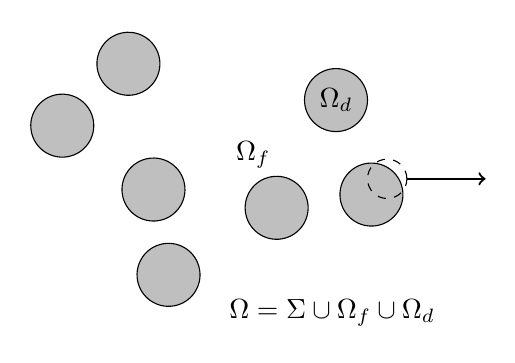
\begin{tikzpicture}
        \foreach \x/\y/\ra/\r/\th in 
        {1/3/0.4/0.4/20,
        2.55/2.7/0.4/0.4/0,
        0.5/0.4/0.4/0.4/10,
        2/1/0.4/0.4/10,
        3/1.5/0.4/0.4/0,
        0.5/1.5/0.4/0.4/10,
        -0.5/2.5/0.4/0.4/10}{
            \draw[fill=gray!50,rotate=\th](\x,\y) ellipse(\ra cm and \ra cm);
        }
        \draw[dashed](3.2,1.7)circle(0.25);
        % \draw[thick,->](3.2,1.7)++(0.1767,0.1767)--++(0.4,0.4)--++(1,0);
        \draw[thick,->](3.2,1.7)++(0.25,0)--++(1,0);
        \draw(2.55,2.7)node{$\Omega_d$};
        \draw(1.5,2)node{$\Omega_f$};
        \draw(2.5,0)node{$\Omega = \Sigma \cup \Omega_f \cup \Omega_d$};
        % \draw(2.5,-1)node{$\Sigma = \sum_\alpha \Sigma_\alpha$};
        % \draw(2.5,-0.5)node{$\Omega_d = \sum_\alpha \Omega_\alpha$};
    \end{tikzpicture}
    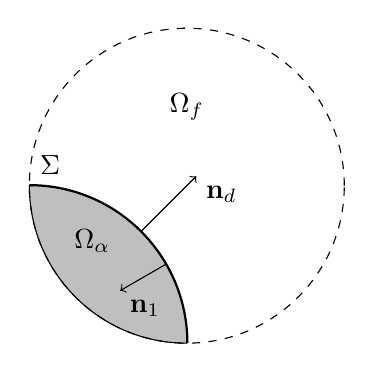
\begin{tikzpicture}%[scale = 0.9]
        \draw[very thick](0:2)arc(0:90:2)node[above right]{$\Sigma$};
        \draw[fill=gray!50](0:2)arc(0:90:2)arc(180:270:2);
        \draw[dashed](2,2)circle(2);
        \draw[->](1.42,1.42)--++(0.7,0.7)node[below right]{$\textbf{n}_d$};
        \draw[->](1.73,1)--++(-0.577,-0.333)node[below right]{$\textbf{n}_1$};
        \draw(2,3)node{$\Omega_f$};
        \draw(0.8,1.3)node{$\Omega_\alpha$};
    \end{tikzpicture}
    \caption{Domain definitions and scheme of the topology of dispersed two-phase flows.
    $\rho_k$ and $\mu_k$ is the density and viscosity of phase $k$, respectively. }
    \label{fig:Scheme}
\end{figure}

The phase and interface indicator functions : 
\begin{align*}
  \chi_k(\textbf{x},t) =  \left\{
    \begin{tabular}{cc}
      $1 \;\text{if} \;\textbf{x} \in \Omega_k(t)$\\
      $0 \;\text{if} \;\textbf{x} \notin \Omega_k(t)$
    \end{tabular}
    \right.
    % \text{for $k = 1,2$},
    % \label{eq:PIF}
    &&
  \delta_I(\textbf{x},t) =  \left\{
    \begin{tabular}{cc}
      $1 \;\text{if} \;\textbf{x} \in \Sigma(t)$\\
      $0 \;\text{if} \;\textbf{x} \notin \Sigma(t)$
    \end{tabular}
    \right.,
    \label{eq:PIF_I}
\end{align*}

\end{frame}



\begin{frame}
  \frametitle{Problem statement: local scale equations.}
  The \underline{mass} ($\rho_f$), \underline{momentum}($\rho_f \textbf{u}_f^0$), and \underline{kinetic energy} ($\rho_f (u_f^0)^2$)  in $\Omega_f$ follow :
\begin{align}
  \div  \textbf{u}_f^0
  &= 
  0
  \\
  \pddt (\rho_f \textbf{u}_f^0)  
  + \div (
      \rho_f \textbf{u}_f^0\textbf{u}_f^0
      - \bm{\sigma}_f^0 
      )
  &= 
  \rho_f \textbf{g}\\
  \pddt [\rho_f/2(u_f^0)^2]  
  + \div [\rho_f/2(u_f^0)^2\textbf{u}_f^0 - \textbf{u}_f^0 \cdot \bm{\sigma}_f^0]
  &=
  \rho_f\textbf{u}_f^0 \cdot \textbf{g}  
  -  \bm{\sigma}_f^0 : \grad \textbf{u}_f^0,
\end{align}
% And at the interfaces : 
% \begin{align*}
%   \Jump {\textbf{u}_k^0}
%   = 0,\;\;\;
%   \Jump {\bm{\sigma}_k^0}
%   = 
%   %  \gamma\kappa\textbf{n}
%   0
%    \;\;\;\; 
%    \text{at} 
%    \;\;\;\; 
%    \Sigma(t)
% \end{align*}
\begin{definition}
  \begin{itemize}
    % \item $\Jump{\ldots} = \sum_k \ldots$ Jump condition.  
    \item The superscript $^0$ indicated that it is a local quantity.
    \item $\rho_k$  density of phase $k$. 
    \item $\textbf{u}_k$  Velocity of phase $k$.
    % \item $\textbf{b}_k^0 = \rho_k \textbf{g}$  local body force.  
    % \item $\gamma$ and $\kappa$  surface tension coefficient and curvature of the surface.  
    \item $\bm\sigma_k^0 = -p_k^0 \textbf{I} + \mu_k (\grad \textbf{u}_k^0+^\dagger\grad \textbf{u}_k^0)$ Newtonian stress tensor of the fluid phase. 
    % \item $\bm\sigma_d^0 = \textbf{Udefined}$ Solid phase stress. 
  \end{itemize}
\end{definition}

\end{frame}


% \begin{frame}
%   \frametitle{Two-fluid formulation of the momentum equation.}
% %   Transport of the phase indicator function, 
% %   \begin{align}
% %     \pddt \chi_k
% %     + \textbf{u}_I^0 \cdot \grad \chi_k
% %     = 0,&&
% % % \end{align}
% % % \begin{align}
% %     \grad \chi_k
% %     = - \delta_I \textbf{n}_k
% %   \end{align}
%   Multiplying the momentum equation by $\chi_k$ gives two-fluid formulation of the momentum equation :
  
%   \begin{align}
%     \label{eq:mass}
%     \pddt (\chi_k\rho_k)  
%     + \div (
%         \chi_k\rho_k \textbf{u}_k^0
%         )
%     &= 0\\
%     \pddt (\chi_k\rho_k \textbf{u}_k^0)  
%     + \div (
%         \chi_k\rho_k \textbf{u}_k^0\textbf{u}_k^0
%         - \chi_k\bm{\sigma}_k^0 
%         )
%     &= 
%     \chi_k\textbf{b}_k^0
%     + \underbrace{\delta_I \bm{\sigma}_k^0\cdot\textbf{n}_k}_\text{Interphase momentum transfer}
%     \label{eq:momentim}
%   \end{align}

%   $\to$ note that (\ref{eq:mass}) and (\ref{eq:momentim}) are defined over $\Omega$ thanks to $\chi_k$. 
%   Therefore, we are now able to apply the ensemble average procedure. 
% \end{frame}



\begin{frame}
  \frametitle{Ensemble average definitions}
Ensemble average (Drew 1983): 
\begin{align*}
  \phi_f (\textbf{x},t) = \avg{\chi_f }\\
  \phi_f \rho_f  \textbf{u}_f (\textbf{x},t) = \avg{\chi_f \rho_f \textbf{u}_f^0 }\\
  \phi_f \bm\sigma_f (\textbf{x},t) = \avg{\chi_f \bm\sigma_f^0 }\\
  % \phi_k \textbf{b}_k (\textbf{x},t) = \avg{\chi_k \textbf{b}_k^0 }
  \label{eq:1_avg}
\end{align*}


\begin{definition}
  \begin{itemize}
    \item $\avg{\ldots}$ ensemble average operator. 
    \item  $\phi_f (\textbf{x},t)$ volume fraction of the phase $f$. 
    \item We dropped the superscript $^0$ on $\textbf{u}^0_k$ to indicate that $\textbf{u}_k$ is a macroscopic quantity. 
    % \item $n_p (\textbf{x},t) = \avg{\sum_\alpha^N \delta(\textbf{x} - \textbf{x}_\alpha(\FF,t))}$ number density of particles. 
    % \item  Both are linked through :   $\phi_d \rho_d= m_p n_p + \frac{1}{2}\grad^2 : (n_p\mathcal{M}_p)+\ldots$
  \end{itemize}
\end{definition}
\end{frame}
\begin{frame}
  \frametitle{Ensemble average definitions}
% Ensemble average: 
% \begin{align*}
%   \phi_f (\textbf{x},t) = \avg{\chi_f }\\
%   \phi_f \rho_f  \textbf{u}_f (\textbf{x},t) = \avg{\chi_f \rho_f \textbf{u}_f^0 }\\
%   \phi_f \bm\sigma_f (\textbf{x},t) = \avg{\chi_f \bm\sigma_f^0 }\\
%   % \phi_k \textbf{b}_k (\textbf{x},t) = \avg{\chi_k \textbf{b}_k^0 }
%   \label{eq:1_avg}
% \end{align*}
Mean kinetic energy of the continuous phase: 
\begin{align*}
  \avg{\rho_f /2 (u_f^0)^2}
  &=
  \rho_f u_f^2
  + 
  \rho_f/2 \avg{\textbf{u}_f'\cdot \textbf{u}_f'}\\
  &=
  \underbrace{\rho_f u_f^2}_\text{Averaged velocity contribution}
  + 
  \underbrace{\rho_f k_f}_\text{Fluctuation velocity contribution}
\end{align*}


\begin{definition}
  \begin{itemize}
    \item $\avg{\ldots}$ ensemble average operator. 
    \item  $\phi_f (\textbf{x},t)$ volume fraction of the phase $f$. 
    \item We dropped the superscript $^0$ on $\textbf{u}^0_k$ to indicate that $\textbf{u}_k$ is a macroscopic quantity. 
    \item $\textbf{u}_f' = \textbf{u}_f^0 - \textbf{u}_f$ velocity fluctuations. 
    % \item $n_p (\textbf{x},t) = \avg{\sum_\alpha^N \delta(\textbf{x} - \textbf{x}_\alpha(\FF,t))}$ number density of particles. 
    % \item  Both are linked through :   $\phi_d \rho_d= m_p n_p + \frac{1}{2}\grad^2 : (n_p\mathcal{M}_p)+\ldots$
  \end{itemize}
\end{definition}
\end{frame}

\begin{frame}{Hybrid formulation}
Long story (Buyevich and Shchelchkova, 1979; Lhuillier, 1992; Zhang and Prosperetti, 1994). Basic idea :

\begin{equation}
  \chi_\alpha f^0_d 
  =\delta_\alpha\intO{f^0_d}
  - \div\left(\delta_\alpha\intO{\textbf{r} f^0_d}\right)
  + \frac{1}{2}\grad\grad :\left(\delta_\alpha\intO{\textbf{rr} f^0_d}\right)-
  \ldots 
  \label{eq:fd_asympt0}
\end{equation}

\begin{equation}
  \delta_{\Gamma\alpha}f_\Gamma^0  
=\delta_\alpha\intS{f^0_\Gamma}
- \div\left(\delta_\alpha\intS{\textbf{r} f^0_\Gamma}\right)
+ \frac{1}{2}\grad\grad :\left(\delta_\alpha\intS{\textbf{rr} f^0_\Gamma}\right)-
\ldots 
\label{eq:fG_asympt0}
\end{equation}
\end{frame}

\begin{frame}
  \frametitle{Averaged continuous phase equations}
\begin{align*}
  &\pddt (\phi_f \rho_f)  
  + \div (
      \phi_f \rho_f\textbf{u}_f
  )
  = 
  0,\\
  &\pddt (\phi_f \rho_f\textbf{u}_f)
  + \div 
      (\phi_f \rho_f\textbf{u}_f\textbf{u}_f)
  = 
  \underbrace{\div \bm\sigma^\text{eff}}_\text{Effective stress}
  + \phi_f \rho_f \textbf{g} 
  - \underbrace{\pSavg{{\bm{\sigma}_f^0 \cdot \textbf{n}_d}}}_\text{Interphase drag force},
\end{align*}
\pause
\underline{Effective stress: } 
\begin{equation*}
  \bm{\sigma}_f^\text{eff}
  =
  - \underbrace{\avg{\chi_f\rho_f\textbf{u}_f'\textbf{u}_f'}}_\text{Reynolds Stress}
  + \underbrace{\phi_f \bm{\sigma}_f}_\text{Mean Newtonian stress}%- n_p \textbf{M}_p
   + \underbrace{ {\pSavg{{\textbf{r}\bm{\sigma}_f^0 \cdot \textbf{n}_d}}}}_\text{Stresslet}
\end{equation*}
\pause

Reynolds stress decomposition: 
\begin{equation}
  \avg{\chi_f\rho_f\textbf{u}_f'\textbf{u}_f'}
  = \text{Deviatoric part}
  + k_f \bm\delta
\end{equation}


\end{frame}


\section{Averaged equations for the pseudo-turbulence stress}

\begin{frame}
  \frametitle{Modeling of $k_f$: first option}

\begin{multline}
  \pddt (\phi_f\rho_fk_f)  
    + \div (
        \phi_f\rho_fk_f\textbf{u}_f
        )
        = \\
      \underbrace{+ \div  \textbf{q}_f^\text{k}}_\text{Effective energy flux}
    - \underbrace{\avg{\chi_f\bm{\sigma}_f^0 : \grad \textbf{u}_f^0}}_\text{Local scale dissipation}
    - \underbrace{\bm{\sigma}_f^\text{eff} : \grad \textbf{u}_f}_\text{Macroscopic dissipation}
    \nonumber \\
    \underbrace{+ (\textbf{u}_f - \textbf{u}_p)\cdot \pSavg{{\bm{\sigma}_f^0 \cdot \textbf{n}_d}} 
    - \pavg{ \textbf{u}_\alpha' \cdot \intS{  \bm{\sigma}_f^0 \cdot \textbf{n}_d}}
    - \pavg{ \intS{\textbf{w}_d^0 \cdot \bm{\sigma}_f^0 \cdot \textbf{n}_d}},}_\text{Work due to the motion of the dispersed phase}
\end{multline}
% \pause
% Effective kinetic enery fluxes
% \begin{align*}
%      \textbf{q}_f^\text{k}
%     =& \rho_f \avg{\chi_f \textbf{u}_f' k_f} 
%     - \avg{\chi_f \textbf{u}_f' \cdot \bm{\sigma}_f^0}
%     + (\textbf{u}_f - \textbf{u}_p)\cdot
%     \pSavg{{\textbf{r}\bm{\sigma}_f^0 \cdot \textbf{n}_d}}\\
%     &
%     - \pavg{ \textbf{u}_\alpha' \cdot \intS{ \textbf{r} \bm{\sigma}_f^0 \cdot \textbf{n}_d}}
%     - \pavg{ \intS{\textbf{r}\textbf{w}_d^0 \cdot \bm{\sigma}_f^0 \cdot \textbf{n}_d}}
%     + \div[\ldots]
% \end{align*}



\begin{definition}
  \begin{itemize}
    \item $\textbf{u}_p$ mean velocity of the droplets center of mass
    \item $\textbf{u}_\alpha$ center of mass velocity of the droplet $\alpha$ 
    \item $\textbf{u}_\alpha' = \textbf{u}_\alpha - \textbf{u}_p$.   
    \item $\textbf{w}_f^0  = \textbf{u}_f^0 - \textbf{u}_\alpha$.  
  \end{itemize}
\end{definition}
\end{frame}

\begin{frame}
  \frametitle{Modeling of $k_f$: first option}

\begin{multline}
  \pddt (\phi_f\rho_fk_f)  
    + \div (
        \phi_f\rho_fk_f\textbf{u}_f
        )
        = 
      + \div  \textbf{q}_f^\text{k}
    - \avg{\chi_f\bm{\sigma}_f^0 : \grad \textbf{u}_f^0}
    - \bm{\sigma}_f^\text{eff} : \grad \textbf{u}_f
    \nonumber \\
    + (\textbf{u}_f - \textbf{u}_p)\cdot \pSavg{{\bm{\sigma}_f^0 \cdot \textbf{n}_d}} 
    - \pavg{ \textbf{u}_\alpha' \cdot \intS{  \bm{\sigma}_f^0 \cdot \textbf{n}_d}}
    - \pavg{ \intS{\textbf{w}_d^0 \cdot \bm{\sigma}_f^0 \cdot \textbf{n}_d}},
\end{multline}
% \pause
Effective kinetic enery fluxes
\begin{align*}
     \textbf{q}_f^\text{k}
    =& \underbrace{\rho_f \avg{\chi_f \textbf{u}_f' k_f} 
    - \avg{\chi_f \textbf{u}_f' \cdot \bm{\sigma}_f^0}}_\text{Turbulent transport and stress transport}\\
    &+ (\textbf{u}_f - \textbf{u}_p)\cdot
    \pSavg{{\textbf{r}\bm{\sigma}_f^0 \cdot \textbf{n}_d}}\\
    &
    \underbrace{- \pavg{ \textbf{u}_\alpha' \cdot \intS{ \textbf{r} \bm{\sigma}_f^0 \cdot \textbf{n}_d}}
    - \pavg{ \intS{\textbf{r}\textbf{w}_d^0 \cdot \bm{\sigma}_f^0 \cdot \textbf{n}_d}}
    + \div[\ldots]}_\text{Energy flux generated due to the motion of the interfaces}
\end{align*}

\end{frame}


\begin{frame}
  \frametitle{Modeling of $k_f$: first option}

\begin{multline}
  \pddt (\phi_f\rho_fk_f)  
    + \div (
        \phi_f\rho_fk_f\textbf{u}_f
        )
        = 
      + \div  \textbf{q}_f^\text{k}
    - \avg{\chi_f\bm{\sigma}_f^0 : \grad \textbf{u}_f^0}
    - \bm{\sigma}_f^\text{eff} : \grad \textbf{u}_f
    \nonumber \\
    + (\textbf{u}_f - \textbf{u}_p)\cdot \pSavg{{\bm{\sigma}_f^0 \cdot \textbf{n}_d}} 
    - \pavg{ \textbf{u}_\alpha' \cdot \intS{  \bm{\sigma}_f^0 \cdot \textbf{n}_d}}
    - \pavg{ \intS{\textbf{w}_d^0 \cdot \bm{\sigma}_f^0 \cdot \textbf{n}_d}},
\end{multline}
\vfill
$\to$ Require numerous closure terms which are either due to \underline{single phase} turbulence or \underline{particle-induced} turbulence. 

\end{frame}


\section{Quasi-steady homogeneous closure for the Reynolds stress}
\begin{frame}
  \frametitle{Modeling of $k_f$: Second option}
Assuming $k_f$ is quasi-steady and nearly homogeneous in space
\begin{equation}
  \pddt (\phi_f\rho_fk_f)  
    + \div (
        \phi_f\rho_fk_f\textbf{u}_f
        )
        \approx 
    %   + \div  \textbf{q}_f^\text{k}
    % - \avg{\chi_f\bm{\sigma}_f^0 : \grad \textbf{u}_f^0}
    % - \bm{\sigma}_f^\text{eff} : \grad \textbf{u}_f
    % \nonumber \\
    % + (\textbf{u}_f - \textbf{u}_p)\cdot \pSavg{{\bm{\sigma}_f^0 \cdot \textbf{n}_d}} 
    % - \pavg{ \textbf{u}_\alpha' \cdot \intS{  \bm{\sigma}_f^0 \cdot \textbf{n}_d}}
    % - \pavg{ \intS{\textbf{w}_d^0 \cdot \bm{\sigma}_f^0 \cdot \textbf{n}_d}},
    0 
\end{equation}
\vfill
$\to$ We can find instead an algebraic solution for $k_f$ or $\avg{\chi_f \textbf{u}_f'\textbf{u}_f'}$. 
\end{frame}


\begin{frame}{Modeling of $k_f$: Second option}
  \textbf{Objective and limiting hypothesis:}
  \begin{equation*}
     \avg{\chi_f \textbf{u}_f'\textbf{u}_f'}
     = 
     \text{Particle induced turbulence}
     + \text{Single phase turbulence}
  \end{equation*}
  \hrule\hrule
  \pause
  \begin{itemize}
    \item 
    Focus on the \textbf{Particle induced turbulence}. 
    \item Assuming : 
    \begin{itemize}
      \item Negligible inertia (\textbf{Stokes} regime)
      \item Dilute regime such that $\phi^{2} \approx 0$ 
      \item Mono-disperse suspension of droplets of radius $a$
    \end{itemize}
  \end{itemize}
\hrule\hrule
$\to$ In this regime the wake of the droplets is the main contribution to  $\avg{\chi_f\textbf{u}_f'\textbf{u}_f'}$ !
\hfill
%\centering
%\href{file:///work/fintzin/BUBLLES_PROJECT/movies/layers.mp4}{\beamergotobutton{Play}}
\end{frame}




\begin{frame}
  \frametitle{Nearest particle statistics} %$\textbf{u}_f^\text{nst}$ and $P_\text{nst}$ }
  \begin{equation*}
    \avg{\chi_f \textbf{u}'_f\textbf{u}'_f}[\textbf{x},t]
        = \phi_f\underbrace{\int 
      \textbf{u}^\text{nst}_f
      \textbf{u}^\text{nst}_f 
      P_\text{nst}(\textbf{r}|\textbf{x}) d\textbf{r} 
    }_\text{Averaged velocity perturbation contribution}
    \mathcal{O}(\phi^2)
    %+ \underbrace{ 
    %  \int \avg{\delta_i h_i \chi_f \textbf{v}_f''\textbf{v}_f''}  d\textbf{r}
    % P_{nst}(\textbf{x},t,\textbf{r}) d\textbf{r}
    %}_{\mathcal{O}(\phi^2)}
  \end{equation*}
  \centering
  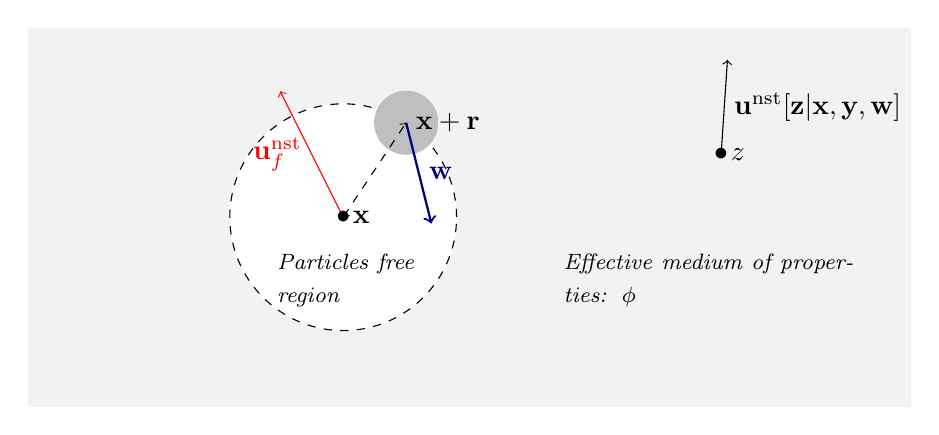
\begin{tikzpicture}[scale=0.8]
    \filldraw[gray!10](-5,-3) rectangle(9,3);
    \filldraw[white](0,0) circle (1.8);
    \filldraw[ gray!10!white](+2.6,0.5)circle (0.5);
    \filldraw[ gray!10!white](-1.5,2.2)circle (0.5);
    \draw[dashed](0:1.8) arc (0:360:1.8);
    % \filldraw[ gray!50!white](0,0) circle (0.5);
    \filldraw[ gray!50!white](1,1.5)circle (0.5);
    \filldraw[ gray!10!white](-0.2,2.5)circle (0.5);
    \draw[->,red](0,0)--++(-1,2)node[midway,left]{$\textbf{u}_f^\text{nst}$};
    \draw(0,0)node{$\bullet$}node[right]{$\textbf{x}$};
    \draw[dashed,<->](0,0)--(1,1.5)node[right]{$\textbf{x}+\textbf{r}$};
    \draw[->,blue!50!black,thick](1,1.5)--++(0.4,-1.6)node[midway,right]{$\textbf{w}$};
    % \draw[dashed](-0.2,3.5);
    \node[text width=2cm] (title) at (0.2,-1) {\footnotesize\textit{Particles free region}};
    % \node[ultra thick] (title) at (-0.5,-1.5) {(\textit{Case 1})};
    \node[text width=4cm] (title) at (6,-1) {\footnotesize\textit{Effective medium of properties:} $\phi$};
    \draw[->] (6,1)node{$\bullet$}node[right]{$z$}--++(0.1,1.5)node[right,midway]{$\textbf{u}^\text{nst}[\textbf{z}|\textbf{x},\textbf{y},\textbf{w}]$};
\end{tikzpicture} 
  

\end{frame}

\begin{frame}
  \frametitle{Single droplet in Stokes flow}

 

  The stokes flow solution of an isolated translating drop is :
  \begin{columns}
    \column{0.6\textwidth}
  \begin{multline*}
    \textbf{u}_f^0
    = \left(\frac{ \textbf{I}}{r} + \frac{\textbf{rr}}{r^3}\right)  \frac{1}{4}\left(\frac{3\lambda + 2}{\lambda +1}\right)  \cdot \textbf{U}\\
    - \left(-\frac{\textbf{I}}{r^3} + \frac{3 \textbf{rr} }{r^5}\right)  \frac{1}{4}\left(\frac{\lambda}{\lambda +1}\right)  \cdot \textbf{U}
  \end{multline*}
  \begin{itemize}
      \item $\lambda$ is the viscosity ratio.
      \item  $\textbf{U} = \textbf{u}_p - \textbf{u}_f$ Mean relative velocity. 
  \end{itemize}
  \column{0.3\textwidth}
  \begin{figure}
    % \caption{Disturbance velocity field of an isolated translating spherical droplet}
    \includegraphics[width=\textwidth]{image/Rising_Stokes.png}
  \end{figure}
  \end{columns}
  


\end{frame}


\begin{frame}
  {
  Pseudo-turbulence in droplet suspension
  }
  \small
  \begin{equation*}
    \avg{\chi_f  \textbf{u}_f' \textbf{u}_f'}
    =
    \underbrace{
      C^{Re}_1(\phi,\lambda)\textbf{UU}
    + C^{Re}_2(\phi,\lambda)U^2 \bm\delta}_\text{Mean particle Induced Turbulence (PIT)}
    %+ \overbrace{C^{Re}_1(\phi,\lambda)\avg{\textbf{u}_p'\textbf{u}_p'}
    %+ C^{Re}_2(\phi,\lambda)\avg{\textbf{u}_{p}'\cdot \textbf{u}_{p}'}\bm\delta
    %}^{\text{Particle center of mass velocity fluctuations}}
    % }_\text{Bubble induced turbulence in a uniform flow}
    % \\
  \end{equation*}
  % \pause
%   \begin{equation*}
%     + \underbrace{\frac{\phi_d a^2 }{105 (\lambda +1)^2 }\left[
%         (129\lambda^2+108\lambda+24)\textbf{E}\cdot \textbf{E}
%         + (20\lambda^2 +20\lambda + 6)
%         (\textbf{E} : \textbf{E})\bm\delta
%     \right]}_\text{Shear Particle Induced Turbulence (S-PIT)}
% \end{equation*}
% \begin{columns}
  % \column{0.5\textwidth}
  \begin{align*}
    C^{Re}_{1} = \frac{9(2+3\lambda)^2 \Gamma(1/3)}{80 (\lambda +1)^2}\phi^{2/3} 
    &&
    C^{Re}_2 = \frac{9(2+3\lambda)^2 \Gamma(1/3)}{80 (\lambda +1)^2}\phi^{2/3} 
    % - \frac{27+82\lambda + 62\lambda^2}{20(\lambda + 1)^2}\phi \right)
  \end{align*}
  \begin{itemize}
    %\item $\avg{\textbf{u}_\alpha'\textbf{u}_\alpha'}$ Particles center of mass velocity fluctuation.  
    \item $\textbf{U} = \textbf{u}_p - \textbf{u}_f$ Mean relative velocity. 
    \item $\lambda$ viscosity ratio between phases
  \end{itemize}
  % \column{0.2\textwidth}
  % \begin{figure}
  %   \caption{Disturbance velocity field of a droplet immersed in a pure linear flow}
%   \end{figure}
%   \column{0.4\textwidth}
%   \includegraphics[width=0.6\textwidth]{image/Shear_Stokes.png}
% \end{columns}
\vfill
\textbf{Semi-empirical} extension of the model !
$C^{Re}_1(\phi, \lambda ) \to C^{Re}_1(\phi, \lambda ,Re) $ 

\end{frame}
\begin{frame}
  \frametitle{Comparison with DNS results and experiments}
  \begin{figure}[h!]
    \centering    
    % \includegraphics[height = 0.25\textwidth]{image/upupexp.png}
    \includegraphics[height = 0.2\textwidth]{image/HOMOGENEOUS_final/CA/cartellier.pdf}
    \includegraphics[height = 0.2\textwidth]{image/HOMOGENEOUS_final/CA/UUyy_Ga_5.pdf}
    \caption{
       Dimensionless vertical component of the Reynolds stress :
       (left) Comparison with the rising bubbles experiment of Cartellier (2009) with $Re \approx 10$. 
       (right) comparison with DNS for two viscosity ratio $\lambda =1,10$ and $Re \approx 1$ DNS. 
    }
    \label{fig:Cp}
\end{figure}  
\begin{itemize}
  \item Good trends in terms of $\phi$ and $\lambda$.  
  \item Quantitative agreement for $\phi < 0.01$.  
\end{itemize}
\end{frame}

\section{Quasi-steady homogeneous closure for the Stresslet}
\begin{frame}{What is the Stresslet ?}
\begin{equation}
  \underbrace{ {\pSavg{{\textbf{r}\bm{\sigma}_f^0 \cdot \textbf{n}_d}}}}_\text{Stresslet} = \bm S + \bm A
\end{equation}
Symmetric part of the first moment ($\bm S$) : $\frac{1}{2} \pSavg{{(\textbf{r}\bm{\sigma}_f^0 + \bm{\sigma}_f^0\textbf{r})\cdot \textbf{n}_d}}$

\begin{block}{Shear dominated flows}
In shear flow the isolated stresslet has a form linear in the rate of strain implies a Newtonian contribution to the bulk stress by the particles. 
This results in the Einstein viscosity $\mu_{\text{eff}} = \mu (1+5/2\phi)$.
\end{block}

\begin{block}{Buoyancy driven flows}
  In the Stokes flow regime, there is no stresslet on a sphere in a uniform flow
\end{block}


%The Stresslet (its deviatoric counterpart) is 
\end{frame}

\begin{frame}{Reciprocal theorem}
\small
  The reciprocal theorem reads (Massoud et Stone 2019).

\begin{align}
 &\int_{S_d+S_\infty} \bm n \cdot \bm \sigma \cdot \hat{ \bm {u}}dS -  \int_{S_d+S_\infty} \bm n \cdot \hat {\bm \sigma} \cdot  \bm {u}dS = \\
 &-Re\int_{V} \hat{ \bm {u}} \cdot \left(\frac{\partial \bm u}{\partial t}+\bm u  \cdot\bm\nabla \bm u \right)dV+\hat{Re}\int_{V} \bm u \cdot \left(\frac{\partial \hat{\bm u}}{\partial t}+\hat{\bm u}  \cdot\bm\nabla \hat{\bm u}\right)dV
\end{align}
where $S_d$ is the drop surface and $S_\infty$ the surface at infinity. The $\hat{}$ denotes the test problem (Stokes flows)
Then, the last integral cancels and we get 
\begin{equation}
    \int_{S_b+S_\infty} \bm n \cdot \bm \sigma \cdot \hat{ \bm {u}}dS -  \int_{S_b+S_\infty} \bm n \cdot \hat {\bm \sigma} \cdot  \bm {u}dS = 
    -Re\int_{V} \hat{ \bm {u}} \cdot \left(\frac{\partial \bm u}{\partial t}+\bm u  \cdot\bm\nabla \bm u \right)dV
    \label{eq:reciprocal}
\end{equation}
Using an appropriately choosen test problem (linear flow past a sphere) one can obtain the first inertial contribution to the stresslet
%We Taylor expand $\bm{u}$ and $\bm \sigma$ as
%\begin{align}
%    \bm{u} &= \bm{u}_0 + Re\bm{u}_1+...\\
%    \bm{\sigma} &= \bm{\sigma}_0 + Re\bm{\sigma}_1+...
%\end{align}

\end{frame}

\begin{frame}
  \frametitle{Stresslet due to the relative motion of the drops}
  \begin{multline}
    \frac{a}{\mu_f U}
    % \left[
        \pSavg{\textbf{r}\bm{\sigma}_f^0 \cdot \textbf{n}_d}
        % - \pOavg{(2 \mu_f \textbf{e}_d^0 - p_f\bm\delta)}
        % \right]
        % \\
    =
     \phi Re C_1
    [
        \textbf{UU} - \frac{1}{3}(U^2)\bm\delta 
    ]
    + Re \phi C_2 (U^2) \bm\delta
    % + \phi p_f \bm\delta
    \label{eq:stresslet_trans}
\end{multline} 
with, 
\begin{align}
    C_1  =  -\frac{63 \lambda^{3} + 150 \lambda^{2} + 112 \lambda + 28}{80 \left(\lambda + 1\right)^{3}}
    &&
    C_2  = \frac{3\lambda^2 + 6\lambda + 4}{48(\lambda +1 )^2}
\end{align}

\end{frame}

%\begin{frame}
%\begin{figure}[h!]
%  \centering
%  \includegraphics[height = 0.25\textwidth]{image/HOMOGENEOUS_final/PA/Sdev_l_1.pdf}
%  \includegraphics[height = 0.25\textwidth]{image/HOMOGENEOUS_final/PA/Sdev_l_10.pdf}
%  \includegraphics[height = 0.25\textwidth]{image/HOMOGENEOUS_final/PA/Sdev_l_100.pdf}
%  \caption{
%      Comparison of the coefficients $-C_1$ (hydrodynamic first moment) and $C_1^{Re}$ (Reynolds stress) appearing in \ref{eq:stress_closed} in terms of the \textit{Reynolds} number based on the mean relative velocity $\textbf{u}_{pf}$ for several volume fractions.
%      Three viscosity ratio are presented: (left) $\lambda = 0.1$ (middle) $\lambda = 1$ (right) $\lambda = 10$. 
%      The density ratio is fixed to $\zeta = 0.9$, and \textit{Bond} number $Bo =0.5$. 
%      (Hollow symbols) Mean coefficient $C_1$ measured with the DNS. 
%      ($\pmb\bigcirc$) $\phi = 0.01$; ($\pmb\triangle$) $ \phi = 0.05$; ($\pmb\square$) $\phi = 0.1$ ($\pmb\lozenge$) $\phi = 0.2$ with $Bo = 0.5$.
%      (dashed line) theoretical formula \ref{eq:stresslet_trans} valid at $\mathcal{O}(Re)$ and $\mathcal{O}(\phi)$. 
%      (Filled symbols) Values of the Reynolds stress constant $C_1^{Re}$ for different volume fraction (indicated by the shape of the symbols) based the DNS results \eqref{chap:pseudoturbulence}. 
%   }
%   \label{fig:Sdev_DNS}
%\end{figure}

%\end{frame}

\begin{frame}
  \frametitle{Conclusion \& Perspectives}

  \begin{enumerate}
    \item The pseudo-turbulent equation for $k_f$ requires a large amount of closure terms. 
    \begin{itemize}
      \item 
      It seems unfeasible (at the present time) to fully close that equations while some closure for the momentum equations are not yet properly accounted for (the stresslet typically). 
    \end{itemize}
    \item If $k_f$ is assumed quasi-steady a model for $\avg{\chi_f\textbf{u}_f'\textbf{u}_f'}$ can be obtained. 
  \end{enumerate}

\end{frame}

\appendix
\transwipe[direction=90]
\begin{frame}{The Nearest Particle Statistics (NPS) approach (DZ Zhang, JFM, 2020)}
  $P_\text{nst}(\textbf{r}|\textbf{x})$ is the probability of finding a nearest particle at \textbf{r} knowing \textbf{x} is occupied by the continuous phase.   

  In the dilute, isotropic and homogeneous regime : 
  \begin{equation*}
    \boxed{P_\text{nst}(\textbf{r}|\textbf{x})
    = \frac{3\phi}{4\pi}
    e^{ - \phi (|\textbf{r}|^3 - 1) }
    \text{ for }
    |\textbf{r}| > a }
  \end{equation*}
  \pause
\begin{columns}
  \column{0.5\textwidth}

\column{0.5\textwidth}
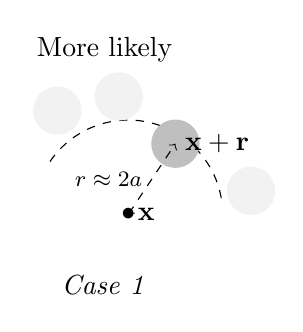
\begin{tikzpicture}[scale=0.6]
  \filldraw[ gray!10!white](+2.6,0.5)circle (0.5);
  \filldraw[ gray!10!white](-1.5,2.2)circle (0.5);
  \draw[dashed](10:2) arc (10:150:2);
  % \filldraw[ gray!50!white](0,0) circle (0.5);
  \filldraw[ gray!50!white](1,1.5)circle (0.5);
  \filldraw[ gray!10!white](-0.2,2.5)circle (0.5);
  \draw(0,0)node{$\bullet$}node[right]{$\textbf{x}$};
  \draw[dashed,<->](0,0)--(1,1.5)node[midway,left]{\footnotesize $r\approx 2 a$}node[right]{$\textbf{x}+\textbf{r}$};
  % \draw[dashed](-0.2,3.5);
  \node[ultra thick] (title) at (-0.5,3.5) {{More likely}};
  \node[ultra thick] (title) at (-0.5,-1.5) {\textit{Case 1}};
\end{tikzpicture} 
\hfill
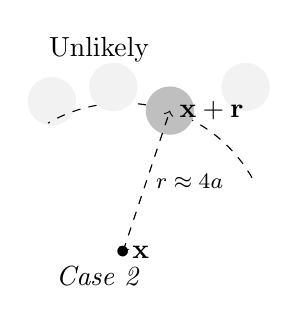
\begin{tikzpicture}[scale=0.6]
  \filldraw[ gray!10!white](+2.6,3.5)circle (0.5);
  \filldraw[ gray!10!white](-1.5,3.2)circle (0.5);
  \draw[dashed](30:3.16) arc (30:120:3.16);
  % \filldraw[ gray!50!white](0,0) circle (0.5);
  \filldraw[ gray!50!white](1,3)circle (0.5);
  \filldraw[ gray!10!white](-0.2,3.5)circle (0.5);
  \draw(0,0)node{$\bullet$}node[right]{$\textbf{x}$};
  \draw[dashed,<->](0,0)--(1,3)node[midway,right]{\footnotesize  $r\approx 4a$}node[right]{$\textbf{x}+\textbf{r}$};
  % \draw[dashed](-0.2,3.5);
  \node[ultra thick] (title) at (-0.5,4.3) {{Unlikely}};
  \node[ultra thick] (title) at (-0.5,-0.5) {\textit{Case 2}};
\end{tikzpicture} 


\end{columns}

\end{frame}


\begin{frame}
  \frametitle{How to find the nearest neighbor velocity field $\textbf{u}_f^{nst}$ ? }
  \centering
  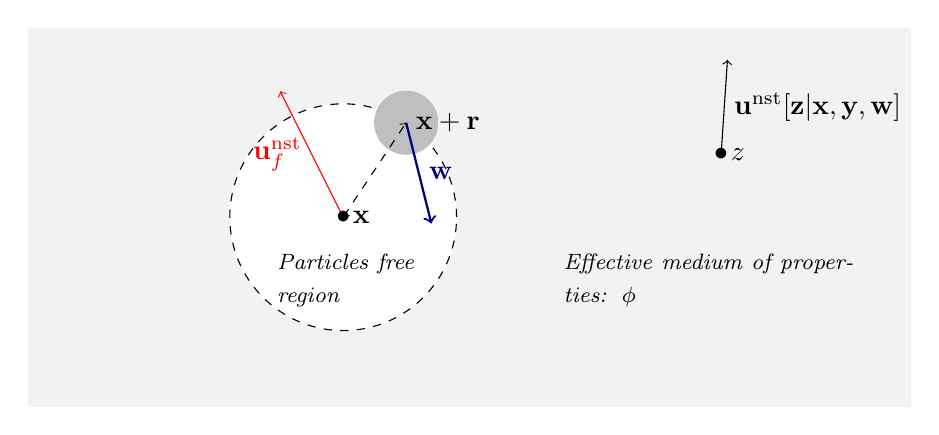
\begin{tikzpicture}[scale=0.8]
    \filldraw[gray!10](-5,-3) rectangle(9,3);
    \filldraw[white](0,0) circle (1.8);
    \filldraw[ gray!10!white](+2.6,0.5)circle (0.5);
    \filldraw[ gray!10!white](-1.5,2.2)circle (0.5);
    \draw[dashed](0:1.8) arc (0:360:1.8);
    % \filldraw[ gray!50!white](0,0) circle (0.5);
    \filldraw[ gray!50!white](1,1.5)circle (0.5);
    \filldraw[ gray!10!white](-0.2,2.5)circle (0.5);
    \draw[->,red](0,0)--++(-1,2)node[midway,left]{$\textbf{u}_f^\text{nst}$};
    \draw(0,0)node{$\bullet$}node[right]{$\textbf{x}$};
    \draw[dashed,<->](0,0)--(1,1.5)node[right]{$\textbf{x}+\textbf{r}$};
    \draw[->,blue!50!black,thick](1,1.5)--++(0.4,-1.6)node[midway,right]{$\textbf{w}$};
    % \draw[dashed](-0.2,3.5);
    \node[text width=2cm] (title) at (0.2,-1) {\footnotesize\textit{Particles free region}};
    % \node[ultra thick] (title) at (-0.5,-1.5) {(\textit{Case 1})};
    \node[text width=4cm] (title) at (6,-1) {\footnotesize\textit{Effective medium of properties:} $\phi$};
    \draw[->] (6,1)node{$\bullet$}node[right]{$z$}--++(0.1,1.5)node[right,midway]{$\textbf{u}^\text{nst}[\textbf{z}|\textbf{x},\textbf{y},\textbf{w}]$};
\end{tikzpicture} 

  Conditionally averaging the stokes equations at a point \textbf{z}, knowing the fluid is present at \textbf{x} with its nearest neighbor at \textbf{y}, yields, 
  \begin{equation*}
    % \pddt \avg{(\delta_\text{nst-f} - P_\text{nst-f})\chi_f}
    \grad \cdot \textbf{u}^\text{nst}
    = 0
    \label{eq:mass_nst_d_stokes}
\end{equation*}
\begin{equation*}
    - \grad p^\text{nst} 
    + \mu_f \grad^2 \textbf{u}^\text{nst}
    = 
    \underbrace{\phi
    \textbf{g}
    \Delta\rho H(|\textbf{r}| - |\textbf{z} - \textbf{x}|)}_\text{particle-free zone buoyancy}
    + \underbrace{\frac{\textbf{w} \mu_f}{a^2} (1 +\grad^2) \delta(\textbf{x}+ \textbf{r} - \textbf{z})}_\text{point forces}
    \label{eq:momentum_nst_d_stokes}
\end{equation*}

\end{frame}

\begin{frame}
  \frametitle{How to find the nearest neighbor velocity field $\textbf{u}_f^{nst}$ ? }

  Conditionally averaging the stokes equations at a point \textbf{z}, knowing the fluid is present at \textbf{x} with its nearest neighbor at \textbf{y}, yields, 
  \begin{equation*}
    % \pddt \avg{(\delta_\text{nst-f} - P_\text{nst-f})\chi_f}
    \grad \cdot \textbf{u}^\text{nst}
    = 0
    \label{eq:mass_nst_d_stokes}
\end{equation*}
\begin{equation*}
    - \grad p^\text{nst} 
    + \mu_f \grad^2 \textbf{u}^\text{nst}
    = 
    \phi
    \textbf{g}
    \Delta\rho H(|\textbf{y} - \textbf{x}| - |\textbf{z} - \textbf{x}|)
    + \frac{\textbf{w} \mu_f}{a^2} (\delta(\textbf{x} - \textbf{y}) +\grad^2\delta)
    \label{eq:momentum_nst_d_stokes}
\end{equation*}

\textbf{The solution : } 
\begin{equation}
  \frac{\textbf{v}^\text{nst}_f}{U}
  =
  \underbrace{\left(\frac{2+3\lambda}{4(1+\lambda)}\right)\textbf{U}\cdot\left[
      1
      +
      \frac{\lambda}{2(2+3\lambda)}\grad^2 
  \right]\mathcal{G}(\textbf{x},\textbf{y})}_\text{particle wake}
  + \underbrace{\phi A |\textbf{x}-\textbf{y}|^2 \textbf{k}}_\text{downstream flow}
  % + \mathcal{O}(\phi). 
  \label{eq:v_nst_solution_adim}
\end{equation}
\begin{equation*}
  \mathcal{G}(\textbf{r})
  = \frac{\bm\delta}{r}
  + \frac{\textbf{rr}}{r^3},
\end{equation*}
\begin{align*}
  \textbf{U} = \textbf{w} - \textbf{u}_f/U
  && 
  \textbf{k} = \textbf{g}/|\textbf{g}|
  &&
  A = \frac{Ga^2}{12 Re}=\frac{\Delta \rho g (2a)^2}{12 \mu_f U}
  \label{eq:A_general}
\end{align*}
\end{frame}

\begin{frame}
  \frametitle{Perspective : a minimal tool to model the continuous phase for buoyant emulsions}


  \begin{align*}
    &\pddt (\phi_f \rho_f)  
    + \div (
        \phi_f \rho_f\textbf{u}_f
    )
    = 
    0,\\
    &\pddt (\phi_f\rho_f \textbf{u}_f)
    + \div (\phi_f\rho_f \textbf{u}_f\textbf{u}_f)
    = \phi_f 
    \left(\div \bm{\Sigma}_f
    + \rho_f \textbf{g}\right)
    + \div  \bm{\sigma}_f^{\text{eff}}
    - \underbrace{n_p \textbf{f}_p}_\text{drag force},
  \end{align*}
  \pause
  
Inter-phase Drag force 
  \begin{align*}
    n_p \textbf{f}_p  
    &= 
    f(Re,\phi, \lambda) \times \textbf{U}
    % \bm{\sigma}_p^{\text{eff}} &= \pavg{\textbf{u}_\alpha'\textbf{u}_\alpha'}
    % 
  \end{align*}
Mean Newtonian stress contribution: 
\begin{align*}
  \bm\Sigma_f &= - p_f \bm\delta + \mu_f [\grad \textbf{u}_f +  (\grad \textbf{u}_f)^\dagger ] 
\end{align*}
Droplets  (or local scale-)  contribution to the stress:
\begin{align*}
    \bm{\sigma}^{\text{eff}}_f 
    &= \underbrace{C_E(Re,\phi,\lambda) \mu_f [\grad \textbf{u}_f +  (\grad \textbf{u}_f)^\dagger ] }_\text{``Einstein viscosity''-like contribution}
    + 
    \underbrace{
      C_1(\phi,\lambda,Re)\textbf{UU}
    + C_2(\phi,\lambda,Re)U^2 \bm\delta}_\text{Mean particle Induced Turbulence (PIT) \& Stresslet}
\end{align*}

\end{frame}
\backmatter




\end{document}
